\subsection{Ballmaschine (Eruieren der Nenndrehzahl)}

\begin{tabular}{p{3.6cm}p{\textwidth-3.6cm-0.7cm}}
\rule{0pt}{11pt}\textit{Typ}              & Ballmaschine \\ 
\rule{0pt}{11pt}\textit{Datum}:           & 06.11.2014   \\
\rule{0pt}{11pt}\textit{Ort}:             & Labor HSLU \\
\rule{0pt}{11pt}\textit{Tester}:          & Matteo, Yves, Pascal\\
\rule{0pt}{11pt}\textit{Ziel des Testes}: & Bestimmung der optimalen Nenndrehzahl der 
Schwungräder sowie die Optimierung des Wurfwinkel.  \\
\rule{0pt}{11pt}\textit{Aufbau / Ablauf}: & In diesem Test wurden zwei DC-Motoren eingesetzt, 
die jeweils von einem  Rohde \& Schwarz Labornetzgerät gespiesen wurde. Die Drehzahl der Motoren 
konnte mittels der Spannung variiert werden. Die Messung der Drehzahl erfolgte über ein berührendes 
Drehzahlmessgerät, das aus dem Physikbestand der Hochschule Luzern ausgeliehen wurde.\\
\rule{0pt}{11pt}\textit{Fazit / Verbesserungs-\newline vorschlag}: & Die Ballzuführung 
muss automatisiert und gleichbleibend sein, damit genaue Aussagen über die Wurfweite 
gemacht werden können. Unterschiedliche Tennisballmarken haben unterschiedliche 
Eigenschaften betreffend Wurfweite -> Fünf Bälle der \enquote{richtigen} Marke kaufen. \\
\end{tabular}
\begin{figure}[h!]
	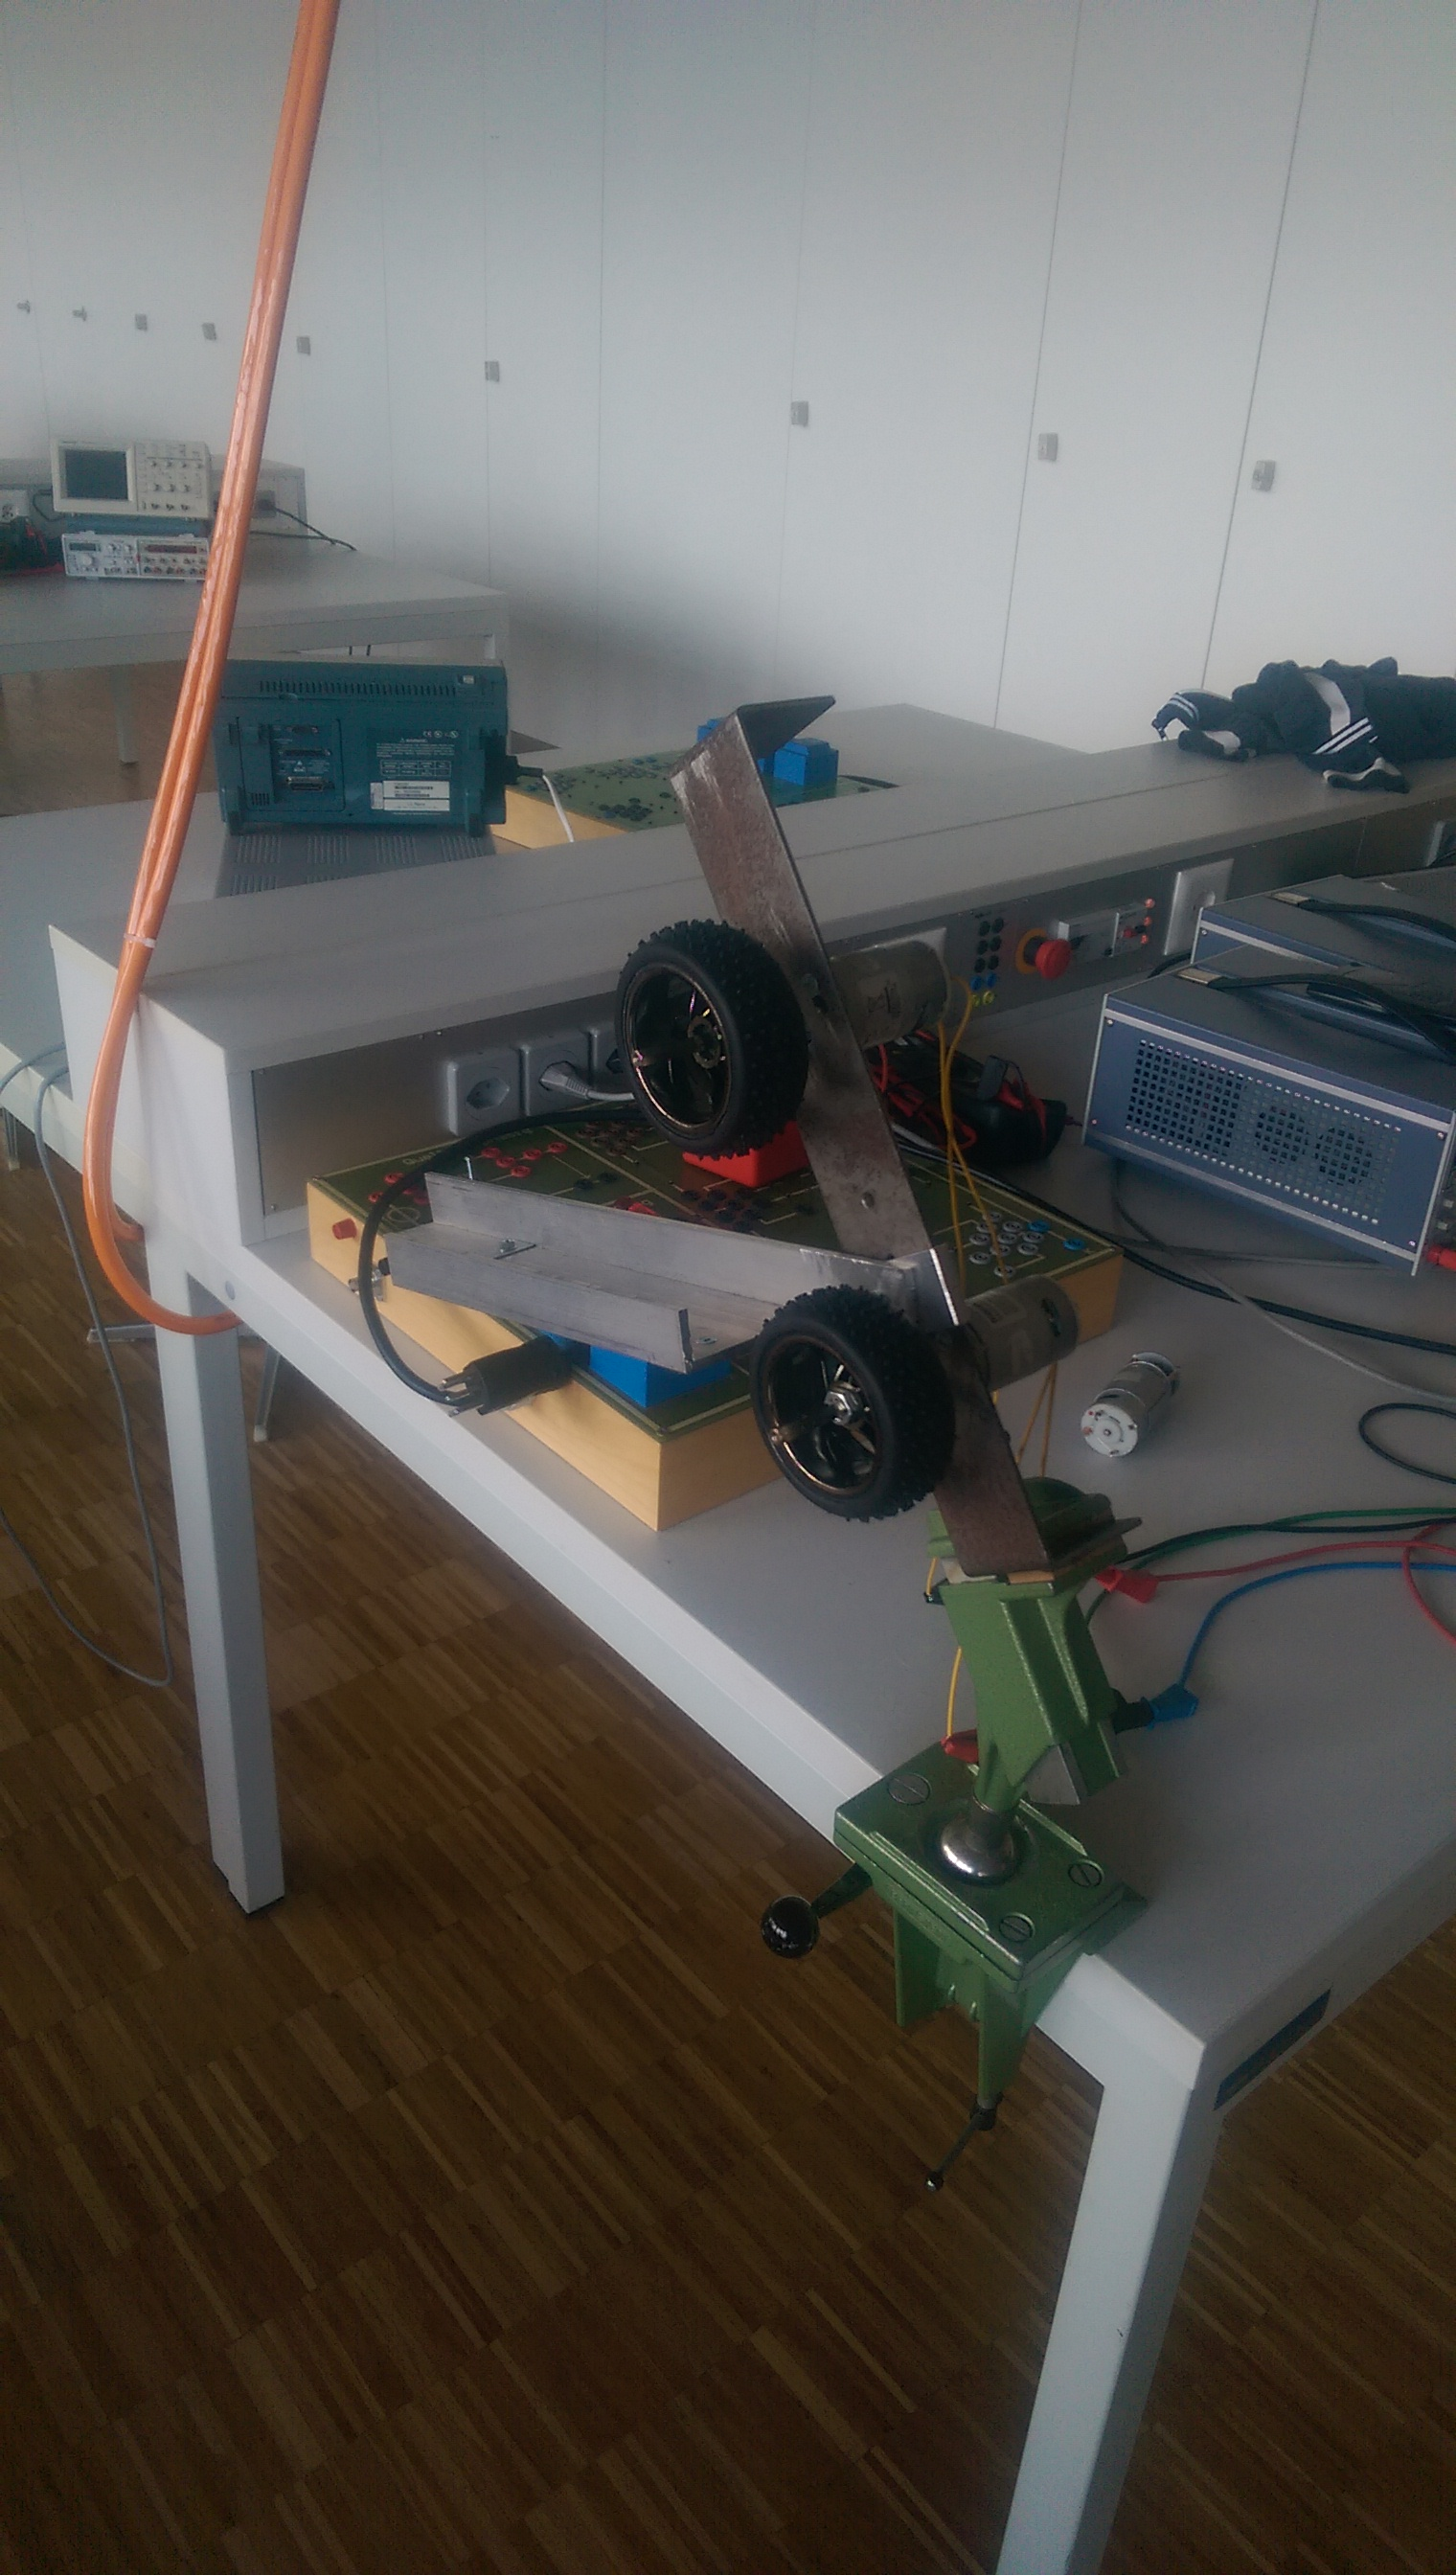
\includegraphics[width=0.7\textwidth,clip,trim=0mm 10cm 0mm 12cm]
	{Funktionstests/Bilder/Ballmaschine_Drehzahl1.jpg}
	\centering
	\caption{Funktionsmuster Ballmaschine} 
\label{abb:Ballmaschine_Drehzahl}
\end{figure}